\documentclass[10pt]{beamer}
\usetheme{metropolis}
\usepackage{appendixnumberbeamer}
\usepackage{booktabs}
\usepackage[scale=2]{ccicons}

\usepackage{pgfplots}
\usepgfplotslibrary{dateplot}

\usepackage{xspace}
\newcommand{\themename}{\textbf{\textsc{metropolis}}\xspace}

\usepackage{hyperref}
\usepackage{pythonhighlight}


\hypersetup{
    bookmarks=true,         % show bookmarks bar?
    unicode=false,          % non-Latin characters in Acrobat’s bookmarks
    pdftoolbar=true,        % show Acrobat’s toolbar?
    pdfmenubar=true,        % show Acrobat’s menu?
    pdffitwindow=false,     % window fit to page when opened
    pdfstartview={FitH},    % fits the width of the page to the window
    pdftitle={My title},    % title
    pdfauthor={Author},     % author
    pdfsubject={Subject},   % subject of the document
    pdfcreator={Creator},   % creator of the document
    pdfproducer={Producer}, % producer of the document
    pdfkeywords={keyword1, key2, key3}, % list of keywords
    pdfnewwindow=true,      % links in new PDF window
    colorlinks=true,       % false: boxed links; true: colored links
    linkcolor=black,          % color of internal links (change box color with linkbordercolor)
    citecolor=green,        % color of links to bibliography
    filecolor=magenta,      % color of file links
    urlcolor=cyan           % color of external links
}

\title{Dive into Redis}
\subtitle{A Quick Look at Redis}
\date{\today}
\author{An{\i}l Can Ayd{\i}n}
\institute{Zetaops}
% \titlegraphic{
\includegraphics[]{img/logo.png}}

\begin{document}

\maketitle

\begin{frame}{Table of contents}
  \setbeamertemplate{section in toc}[sections numbered]
  \tableofcontents[hideallsubsections]
\end{frame}

\section{Introduction}
\begin{frame}[fragile]{About}
  \begin{itemize}
    \item \href{http://www.iyte.edu.tr/}{Izmir Institute of Technology} - \href{http://arf.iyte.edu.tr/}{Computer Engineering}
      \begin{itemize}
        \item B.Sc. 2010 - 2016
        \item M.Sc  2016 - Ongoing
          \begin{itemize}
            \item \textbf{Interests:} Biometric Recognition, Image Processing, Artificial
            Intelligence, Machine Learning, Neural Networks
          \end{itemize}
      \end{itemize}
    \item Sava Consultancy, Izmir.
      \begin{itemize}
        \item Android Developer 2015 - 2016, Part-time
      \end{itemize}
    \item \href{http://zetaops.io/}{Zetaops}, Izmir.
      \begin{itemize}
          \item Software Developer 2017 - Ongoing
            \begin{itemize}
              \item \textbf{Interests:} Problem Solving, High Availability, Scalability,
              RESTful API Design, Data Modeling, Caching, Microservices
              \item \textbf{Stack:} Python, RabbitMQ, Redis, Riak
            \end{itemize}
      \end{itemize}
    \item Trying to:
      \begin{itemize}
        \item keep up with the state-of-the-art tech
        \item learn continuosly to be able to see the next level of this
        challenging game which we all trying to survive in it
        \item contribute open source projects to make the world a better place
        \item wake up early to catch things up, couldn't make it yet
      \end{itemize}
  \end{itemize}
\end{frame}

\begin{frame}[fragile]{Contact}
  Find me on
  \begin{itemize}
    \item \href{https://github.com/anlcnydn}{github/anlcnydn}
    \item \href{https://twitter.com/anlcnydn}{twitter/anlcnydn}
  \end{itemize}
  or mail me at \href{mailto:anil@zetaops.io}{anil@zetaops.io}
\end{frame}

\begin{frame}[fragile]{Links}
  \begin{itemize}
    \item \href{https://github.com/anlcnydn/gdg2017-dive-into-redis}{github/anlcnydn/gdg2017-dive-into-redis}
    \item \href{https://github.com/anlcnydn/gdg2017-slides}{github/anlcnydn/gdg2017-slides}
  \end{itemize}
\end{frame}

\section{Overview on Caching and Redis}

\begin{frame}[fragile]{Caching}
  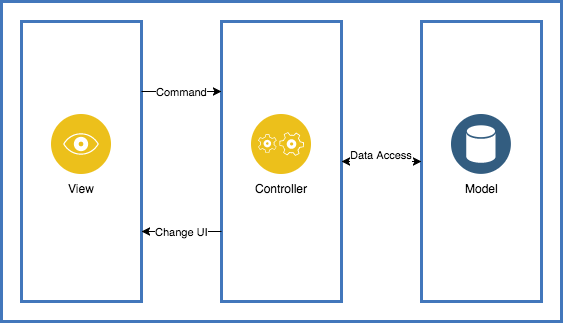
\includegraphics[scale=0.5]{img/mvc-classic}
\end{frame}

\begin{frame}[fragile]{Caching}
  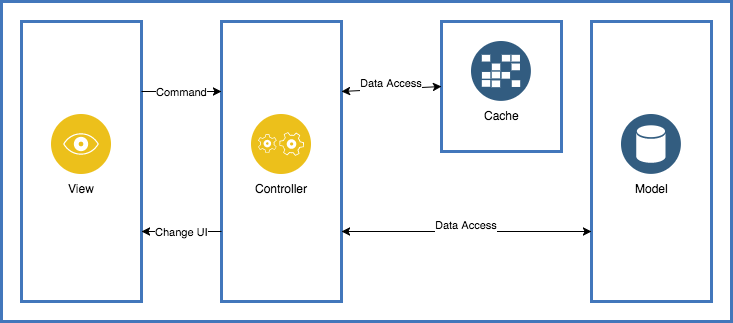
\includegraphics[scale=0.4]{img/mvc-cache}
\end{frame}

\begin{frame}[fragile]{Caching}
  \begin{itemize}
    \item Improves scalability by distributing query workload
    \item Allows flexibility in the processing of data
    \item Caching can improve availability of data
    \item Improved data access speeds
  \end{itemize}
\end{frame}

\begin{frame}[fragile]{Why Redis}
  \begin{itemize}
    \item Open source
    \item In-memory data structure store, used as database, cache and message
    broker
    \item Provides high performance and low latency
    \item Blazingly fast
    \item Written in C
    \item Optimized to handle millions of operations in a second with less than
    1 ms latency in a single server
    \item Pre-built data structures
    \item Client libraries in almost every language and active developer
    community and contributors
  \end{itemize}
\end{frame}

\begin{frame}[fragile]{Redis}
  \begin{itemize}
    \item redis-cli
    \item \href{https://github.com/andymccurdy/redis-py}{redis-py}
  \end{itemize}

\end{frame}

\section{Redis Data Types}

\begin{frame}[fragile]{Data Types}
  Not a \textit{plain} key-value store, it is actually a \textit{data structures
   server}

  List of all the data structures supported by Redis:
  \begin{itemize}
		\item Binary-safe strings.
		\item Lists: sorted order of insertion, linked lists.
		\item Sets: unique, unsorted
    \item Sorted sets: Sorted by their \textbf{score}. Unlike Sets it is
    possible to retrieve a range of elements (for example you may ask: give me
    the top 10, or the bottom 10).
    \item Hashes, map, dict
    \item Bit arrays (or simply bitmaps): it is possible, using special commands,
    to handle String values like an array of bits
    \item HyperLogLogs: this is a probabilistic data structure which is used in
    order to estimate the cardinality of a set, also not in the scope of this
    presentation.
	\end{itemize}
\end{frame}

\subsection{Keys and Strings}

\begin{frame}[fragile]{Redis Keys}
  \begin{itemize}
    \item Redis keys are binary safe, this means that you can use any binary
    sequence as a key
    \item Very long keys are not a good idea.
      \begin{itemize}
        \item Not memory efficient.
        \item May increase the burden of the key look-up.
      \end{itemize}
    \item Very short keys are often not a good idea. user:1000:followers beats
    u1000flw.
    \item Try to stick with a schema. object-type:id is a good idea, user:1000.
    \item The maximum allowed key size is 512 MB.
  \end{itemize}
\end{frame}

\begin{frame}[fragile]{Strings}
  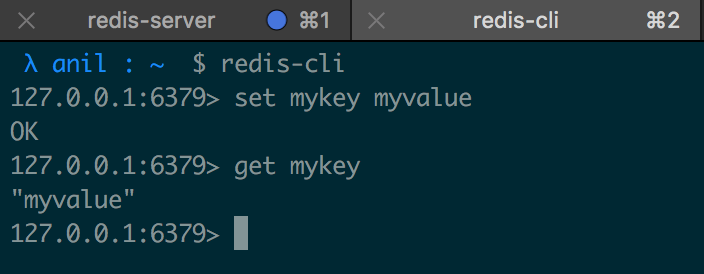
\includegraphics[scale=0.9]{img/redis-basic-set-get}
\end{frame}

\begin{frame}[fragile]{SET and GET in redis-py}
  \inputpython{redis.py}{19}{26}
\end{frame}

\begin{frame}[fragile]{SET}
  \begin{itemize}
    \item Note that SET will replace any existing value already stored into
    the key
    \item Values can be strings (including binary data) of every kind, for
    instance you can store a jpeg image inside a value.
    \item A value can't be bigger than 512 MB.
    \item The SET command has interesting options, that are provided as
    additional arguments.
    \item For example, I may ask SET to fail if the key already exists, or the
    opposite, that it only succeed if the key already exists.
  \end{itemize}
\end{frame}

\begin{frame}[fragile]{NX and XX}
  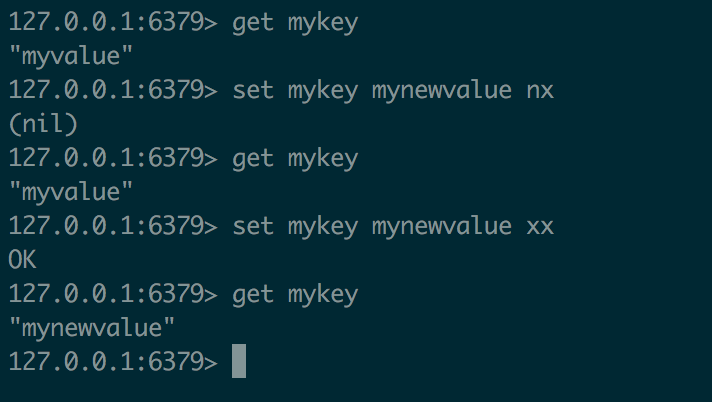
\includegraphics[scale=0.9]{img/set-get-advanced}
\end{frame}

\begin{frame}[fragile]{NX and XX in redis-py}
  \inputpython{redis.py}{30}{43}
\end{frame}


\begin{frame}[fragile]{INCR}
  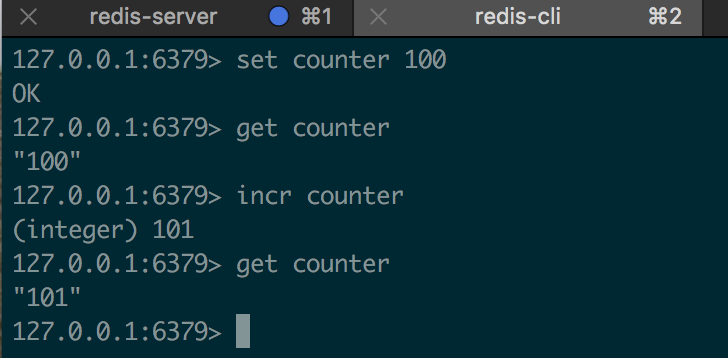
\includegraphics[scale=0.9]{img/incr}
\end{frame}

\begin{frame}[fragile]{INCR in redis-py}
  \inputpython{redis.py}{47}{53}
\end{frame}


\begin{frame}[fragile]{INCR, INCRBY, DECR and DECRBY}
    All are atomic. No race condition.
\end{frame}

\begin{frame}[fragile]{GETSET}
    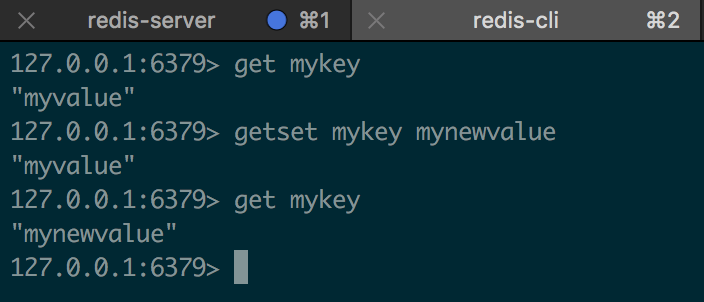
\includegraphics[scale=0.9]{img/getset}
\end{frame}

\begin{frame}[fragile]{GETSET Case Story}
  If you have a system that increments a Redis key using INCR every time your
  web site receives a new visitor. You may want to collect this information
  once every hour, without losing a single increment. You can GETSET the key,
  assigning it the new value of "0" and reading the old value back.
\end{frame}

\begin{frame}[fragile]{MSET and MGET}
    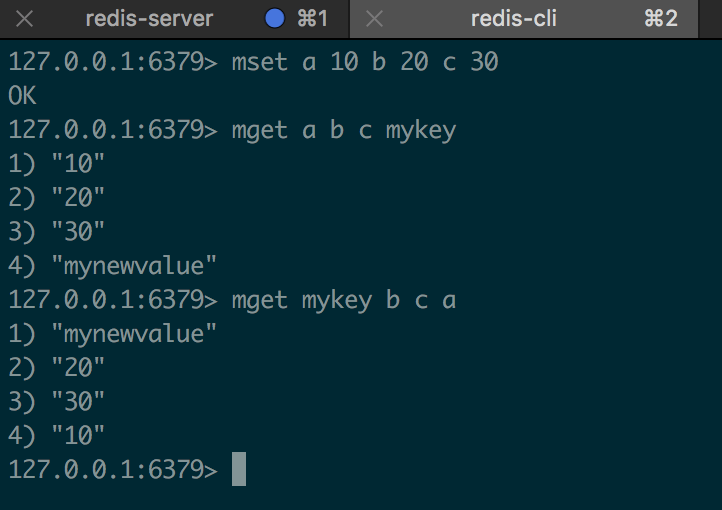
\includegraphics[scale=0.9]{img/mset-mget}
\end{frame}

\begin{frame}[fragile]{EXISTS and DEL}
    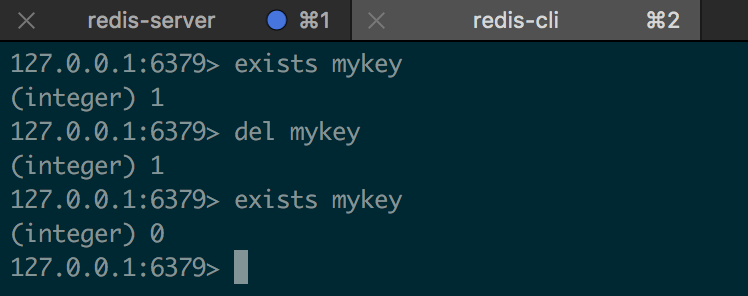
\includegraphics[scale=0.7]{img/del-exists}
\end{frame}

\subsection{Lists}

\begin{frame}[fragile]{Lists}
  \begin{itemize}
    \item Redis lists are implemented via Linked Lists
    \item The operation of adding a new element in the head or in the tail of
    the list is performed in constant time.
    \item What's the downside? Accessing an element by index is very fast in
    lists implemented with an Array (constant time indexed access) and not so
    fast in lists implemented by linked lists (where the operation requires an
    amount of work proportional to the index of the accessed element).
    \item When fast access to the middle of a large collection of elements is
    important, there is a different data structure that can be used, called
    sorted sets.
  \end{itemize}
\end{frame}

\begin{frame}[fragile]{First Steps with Lists}
  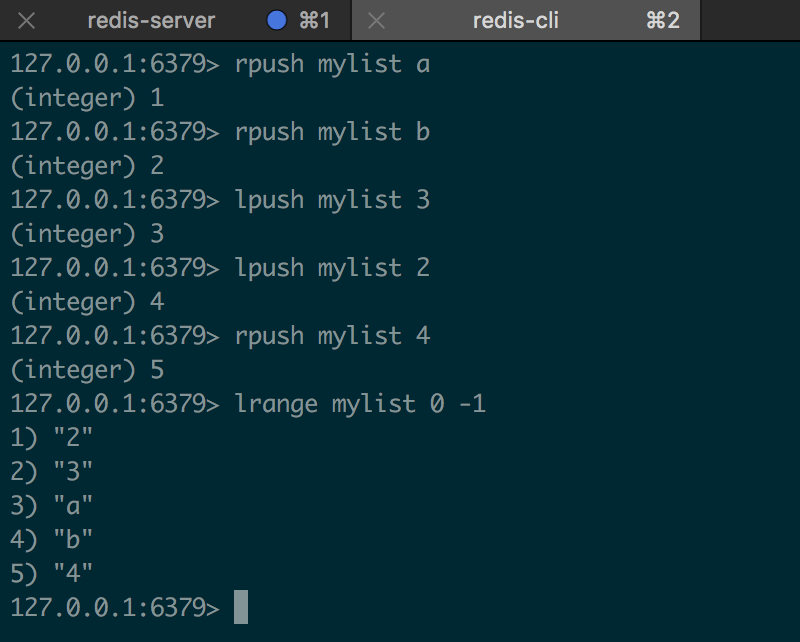
\includegraphics[scale=0.7]{img/lpush-rpush-lrange}
\end{frame}

\begin{frame}[fragile]{LRANGE}
  \begin{itemize}
    \item Note that LRANGE takes two indexes, the first and the last element
    of the range to return. Both the indexes can be negative, telling Redis to
    start counting from the end: so -1 is the last element, -2 is the
    penultimate element of the list, and so forth
    \item LPUSH and RPUSH are variadic commands, meaning that you are free to
    push multiple elements into a list in a single call
    \item You can pop elements from left and right, similarly to how you can
    push elements in both sides of the list
  \end{itemize}
\end{frame}

\begin{frame}[fragile]{LPOP and RPOP}
  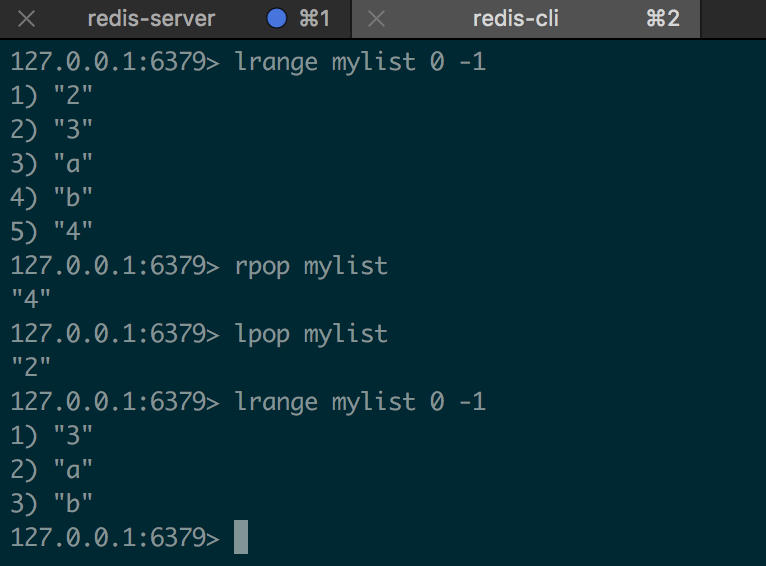
\includegraphics[scale=0.8]{img/pop}
\end{frame}

\begin{frame}[fragile]{Common Use Cases for Lists}
  \begin{itemize}
    \item Remember the latest updates posted by users into a social network
    \item Communication between processes, using a producer-consumer pattern
    where the producer pushes items into a list, and a consumer (usually a
    worker) consumes those items and executed actions. Redis has special list
    commands to make this use case both more reliable and efficient.
    \item For example both the popular Ruby libraries
    \href{https://github.com/resque/resque}{resque} and
    \href{https://github.com/mperham/sidekiq}{sidekiq} use Redis lists under
    the hood in order to implement background jobs
    \item The popular Twitter social network
    \href{https://www.infoq.com/presentations/Real-Time-Delivery-Twitter}{takes the latest tweets}
    posted by users into Redis lists.
  \end{itemize}
\end{frame}

\begin{frame}[fragile]{Capped Lists}
  \begin{itemize}
    \item Redis allows us to use lists as a capped collection, only remembering
    the latest N items and discarding all the oldest items using the LTRIM
    command.
    \item The LTRIM command is similar to LRANGE, but instead of \textbf{displaying
    the specified range of elements} it sets this range as the new list value.
    All the elements outside the given range are removed.
  \end{itemize}
\end{frame}

\begin{frame}[fragile]{LTRIM}
  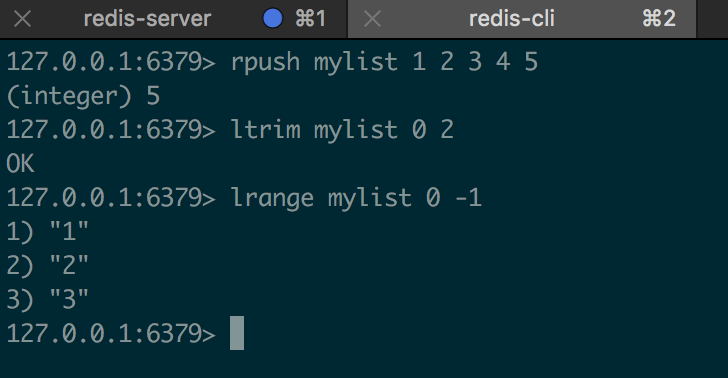
\includegraphics[scale=0.9]{img/ltrim}
\end{frame}

\begin{frame}[fragile]{Blocking Operations on Lists}
  \begin{itemize}
    \item The usual producer/consumer setup
    \item To push items into the list, producers call LPUSH
    \item To extract/process items from the list, consumers call RPOP
    \item If the list is empty and there is nothing to process, so RPOP just
    returns NULL
    \item In this case a consumer is forced to wait some time and retry again
    with RPOP
    \item This is called polling, and is not a good idea
  \end{itemize}
\end{frame}

\begin{frame}[fragile]{BRPOP and BLPOP}
  BRPOP and BLPOP are versions of RPOP and LPOP able to block if the list is
  empty: they'll return to the caller only when a new element is added to the
  list, or when a user-specified timeout is reached.
\end{frame}

\begin{frame}[fragile]{BRPOP}
  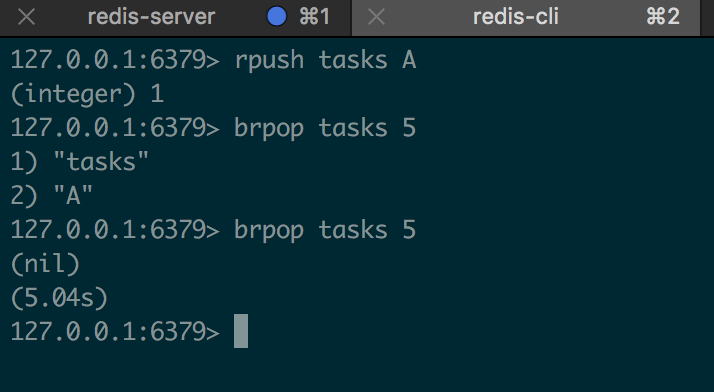
\includegraphics[scale=0.9]{img/brpop}
\end{frame}

\begin{frame}[fragile]{More on BRPOP}
  \begin{itemize}
    \item Note that you can use 0 as timeout to wait for elements forever, and
    you can also specify multiple lists and not just one, in order to wait on
    multiple lists at the same time, and get notified when the first list
    receives an element.
    \item Clients are served in an ordered way: the first client that blocked
    waiting for a list, is served first when an element is pushed by some other
    client, and so forth.
    \item The return value is different compared to RPOP: it is a two-element
    array since it also includes the name of the key, because BRPOP and BLPOP
    are able to block waiting for elements from multiple lists.
    \item If the timeout is reached, NULL is returned.
    \item Suggested reading on \href{https://redis.io/commands/rpoplpush}{RPOPLPUSH}
    and \href{https://redis.io/commands/brpoplpush}{BRPOPLPUSH}
  \end{itemize}
\end{frame}

\begin{frame}[fragile]{Automatic Creation and Removal of Keys}
  \begin{itemize}
    \item When we add an element to an aggregate data type, if the target key
    does not exist, an empty aggregate data type is created before adding the
    element.
    \item When we remove elements from an aggregate data type, if the value
    remains empty, the key is automatically destroyed.
    \item Calling a read-only command such as LLEN (which returns the length of
    the list), or a write command removing elements, with an empty key, always
    produces the same result as if the key is holding an empty aggregate type
    of the type the command expects to find.
  \end{itemize}
\end{frame}

\subsection{Hashes}

\begin{frame}[fragile]{HMSET, HGET, HGETALL}
  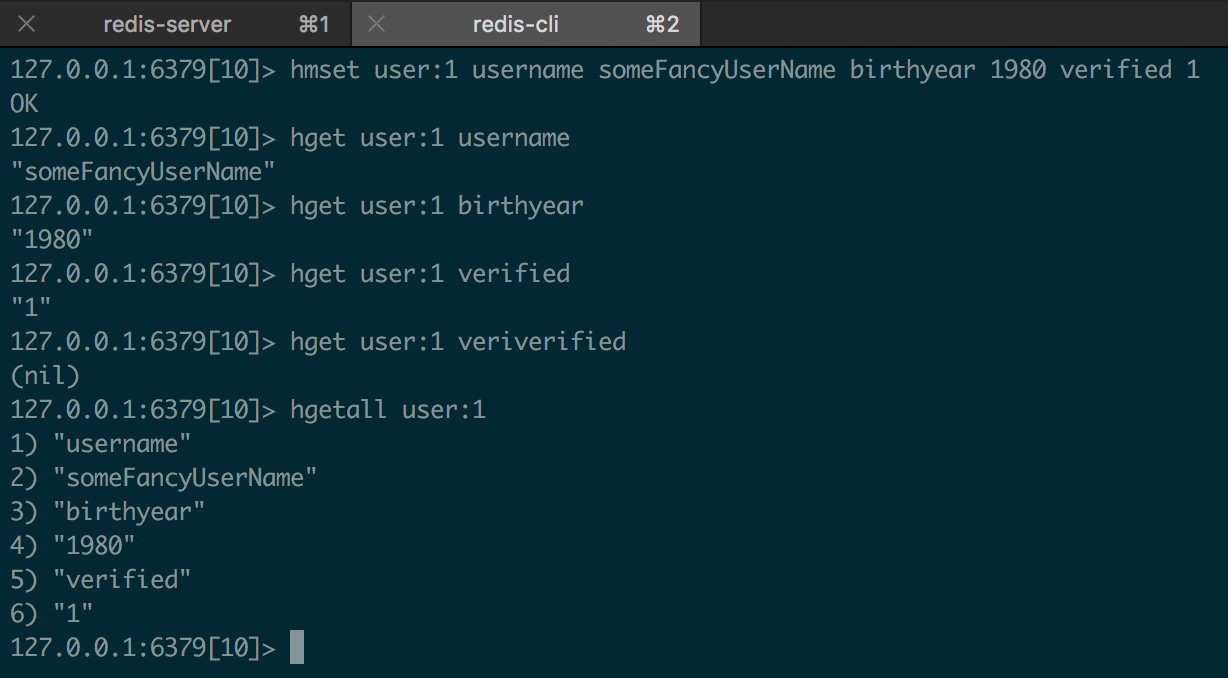
\includegraphics[scale=0.5]{img/hmset-hget-hgetall}
\end{frame}

\begin{frame}[fragile]{HMGET}
  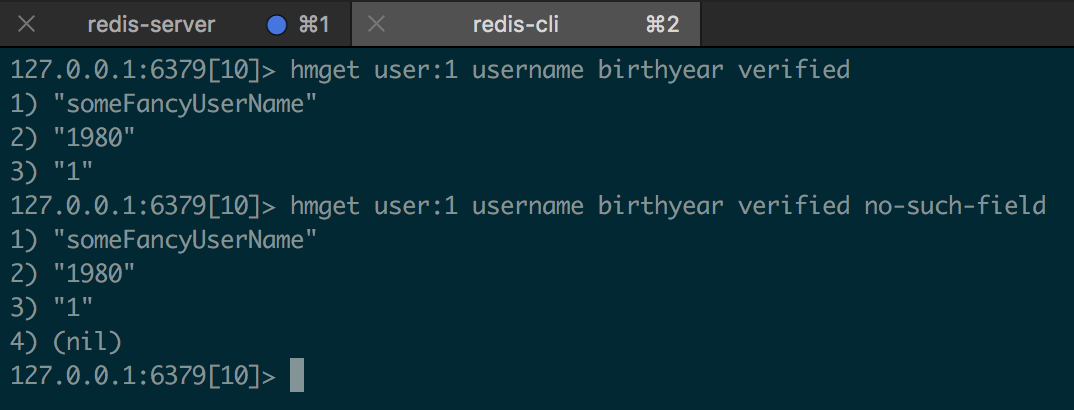
\includegraphics[scale=0.5]{img/hmget}
\end{frame}

\begin{frame}[fragile]{More on Hashes}
  While hashes are handy to represent objects, actually the number of fields
  you can put inside a hash has no practical limits (other than available
  memory), so you can use hashes in many different ways inside your application.

  \href{https://redis.io/commands#hash}{More} on hashes.
\end{frame}

\subsection{Sets}

\begin{frame}[fragile]{Sets}
  \begin{itemize}
    \item Redis Sets are unordered collections of strings
    \item The SADD command adds new elements to a set.
    \item It's also possible to do a number of other operations against sets
    like testing if a given element already exists, performing the intersection,
    union or difference between multiple sets, and so forth.
  \end{itemize}
\end{frame}

\begin{frame}[fragile]{SADD}
  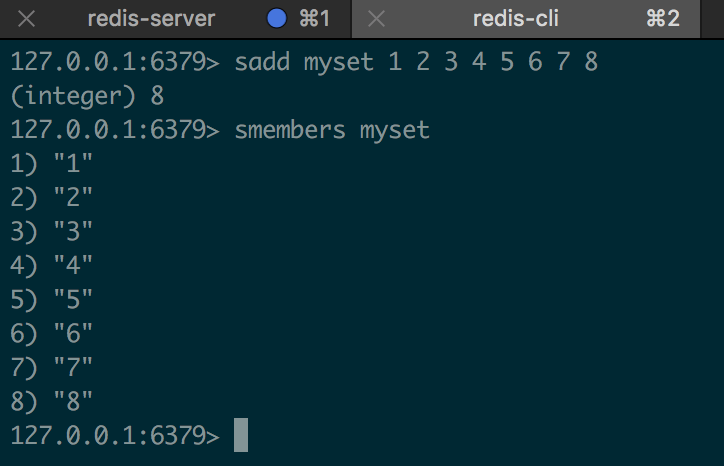
\includegraphics[scale=0.9]{img/sadd}
\end{frame}

\begin{frame}[fragile]{SINTER}
  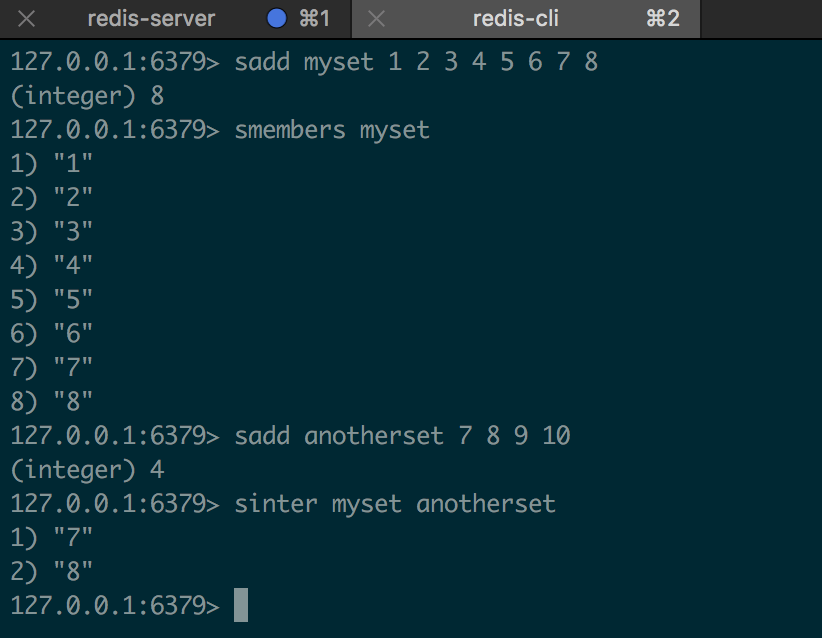
\includegraphics[scale=0.7]{img/sinter}
\end{frame}

\begin{frame}[fragile]{SUNIONSTORE}
  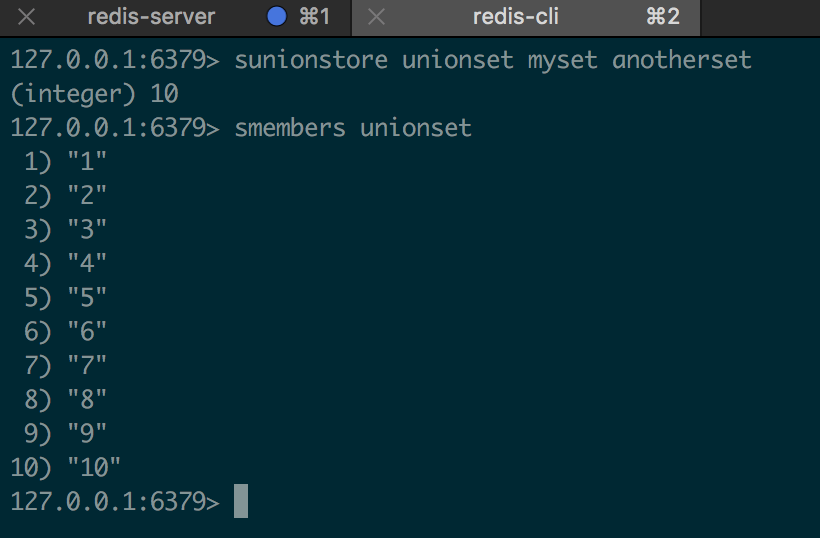
\includegraphics[scale=0.7]{img/sunionstore}
\end{frame}

\begin{frame}[fragile]{SPOP and SCARD}
  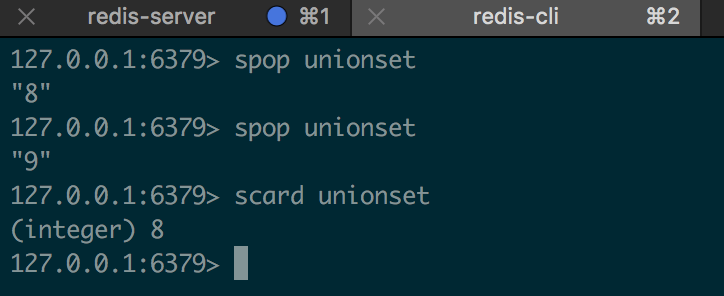
\includegraphics[scale=0.7]{img/spop-scard}
\end{frame}

\begin{frame}[fragile]{SRANDMEMBER}
  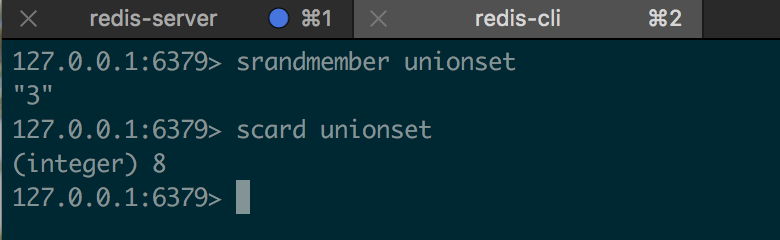
\includegraphics[scale=0.7]{img/srandmember}
\end{frame}

\begin{frame}[fragile]{Sorted Sets}
  \begin{itemize}
    \item Sorted sets are a data type which is similar to a mix between a Set
    and a Hash
    \item Like sets, sorted sets are composed of unique, non-repeating string
    elements, so in some sense a sorted set is a set as well
    \item However while elements inside sets are not ordered, every element in
    a sorted set is associated with a floating point value, called the score
    (this is why the type is also similar to a hash, since every element is
    mapped to a value)
    \item Moreover, elements in a sorted sets are taken in order (so they are
    not ordered on request, order is a peculiarity of the data structure used
    to represent sorted sets).
  \end{itemize}
\end{frame}

\begin{frame}[fragile]{Sorted Sets: Ordering Rules}
  They are ordered according to the following rule:
  \begin{itemize}
    \item If A and B are two elements with a different score, then A $>$ B if
    A.score is $>$ B.score.
    \item If A and B have exactly the same score, then A $>$ B if the A string is
    lexicographically greater than the B string. A and B strings can't be equal
    since sorted sets only have unique elements.
  \end{itemize}
\end{frame}

\begin{frame}[fragile]{ZADD}
  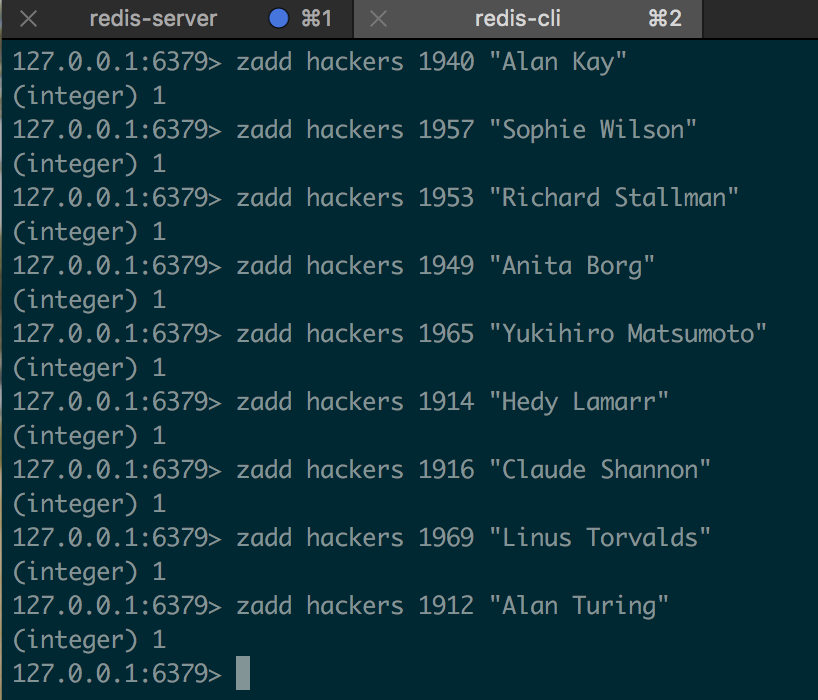
\includegraphics[scale=0.6]{img/zadd}
\end{frame}

\begin{frame}[fragile]{ZRANGE}
  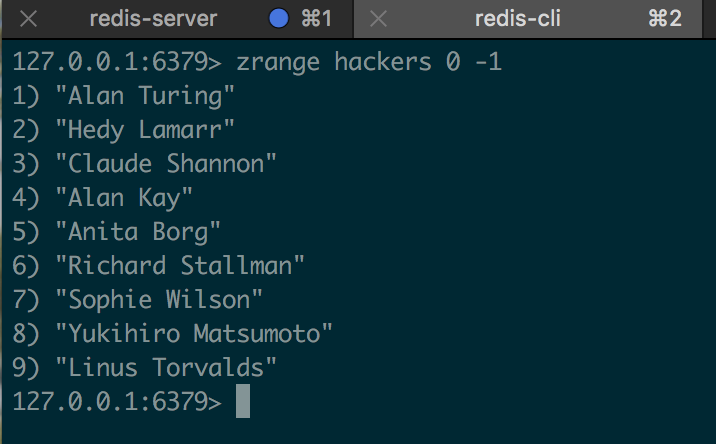
\includegraphics[scale=0.8]{img/zrange}
\end{frame}

\begin{frame}[fragile]{More on Sorted Sets}
  \begin{itemize}
    \item With sorted sets it is trivial to return a list of hackers sorted by
    their birth year because actually they are already sorted.
    \item Implementation note: Sorted sets are implemented via a dual-ported
    data structure containing both a skip list and a hash table, so every time
    we add an element Redis performs an O(log(N)) operation.
    That's good, but when we ask for sorted elements Redis does not have to do
    any work at all, it's already all sorted.
    \item What if I want to order them the opposite way, youngest to oldest?
    Use ZREVRANGE instead of ZRANGE
    \item It is possible to return scores as well, using the WITHSCORES argument
  \end{itemize}
\end{frame}

\begin{frame}[fragile]{Operating on Ranges: ZRANGEBYSCORE}
  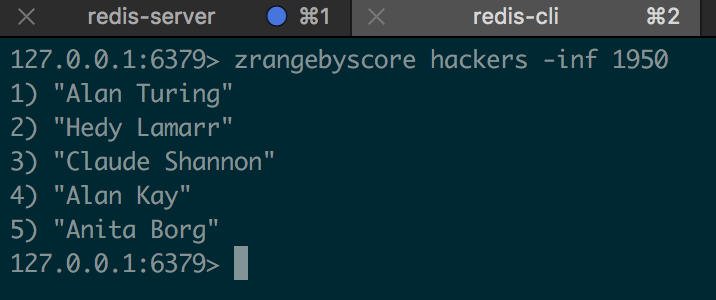
\includegraphics[scale=0.8]{img/zrangebyscore}
\end{frame}

\begin{frame}[fragile]{Operating on Ranges: ZREMRANGEBYSCORE}
  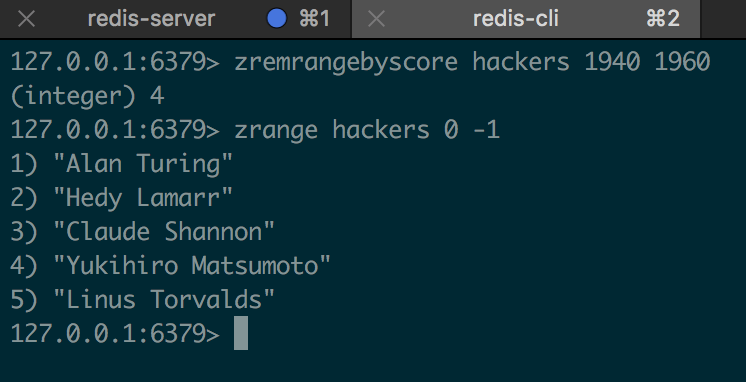
\includegraphics[scale=0.8]{img/zremrangebyscore}
\end{frame}

\begin{frame}[fragile]{Operating on Ranges: ZRANK and ZREVRANK}
  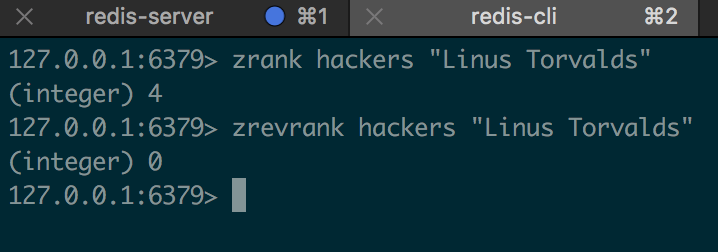
\includegraphics[scale=0.8]{img/zrank-zrevrank}
\end{frame}

\begin{frame}[fragile]{Lexicographical Scores: ZRANGEBYLEX}
  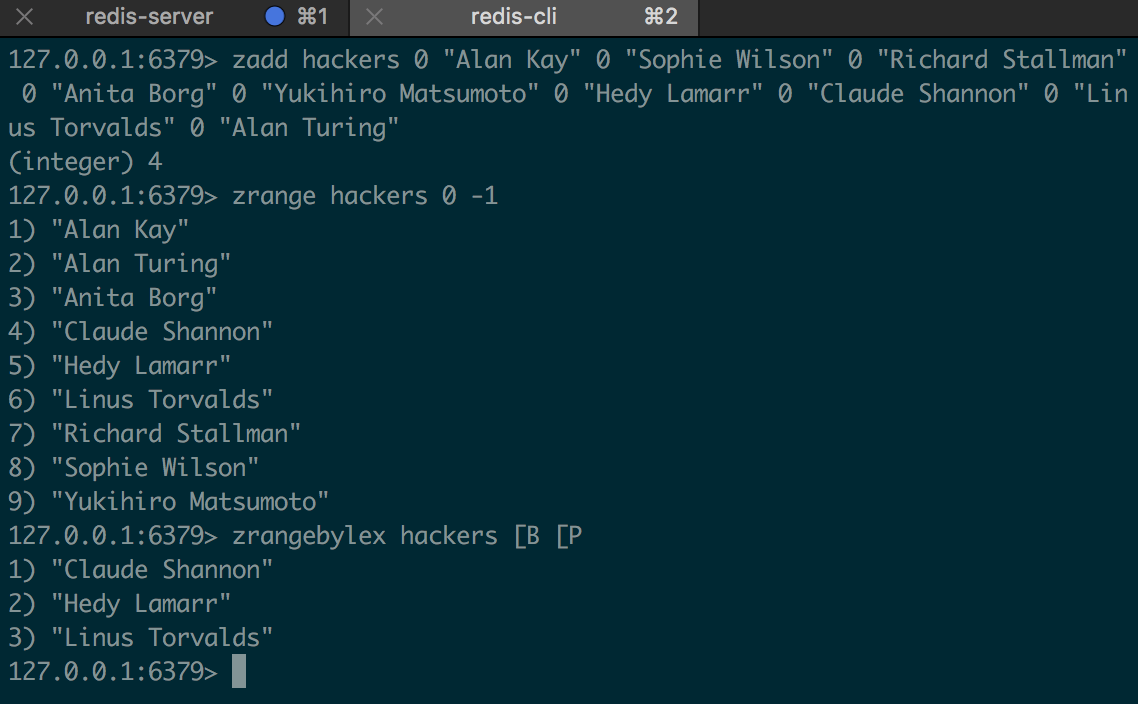
\includegraphics[scale=0.5]{img/zrangebylex}
\end{frame}

\subsection{Bitmaps}

\begin{frame}[fragile]{Bitmaps}
  Bitmaps are not an actual data type, but a set of bit-oriented operations
  defined on the String type.
\end{frame}

\subsection{Data Types Conclusion}

\begin{frame}{Data Types Conclusion}
  \begin{itemize}
		\item Binary-safe strings.
		\item Lists
		\item Sets
    \item Sorted sets
    \item Hashes
    \item Bitmaps
	\end{itemize}
\end{frame}

\section{Redis Pipelining}
\begin{frame}[fragile]{Request/Response protocol}
  Redis is a TCP server using the client-server model and what is called
  a Request/Response protocol \footnote{\href{https://redis.io/topics/clients}{
  Redis Clients Handling}}.

  This means that usually a request is accomplished with the following steps:
  \begin{itemize}
    \item The client sends a query to the server, and reads from the socket,
    usually in a blocking way, for the server response.
    \item The server processes the command and sends the response back to
    the client.
  \end{itemize}
\end{frame}

\begin{frame}[fragile]{Request/Response protocol}
  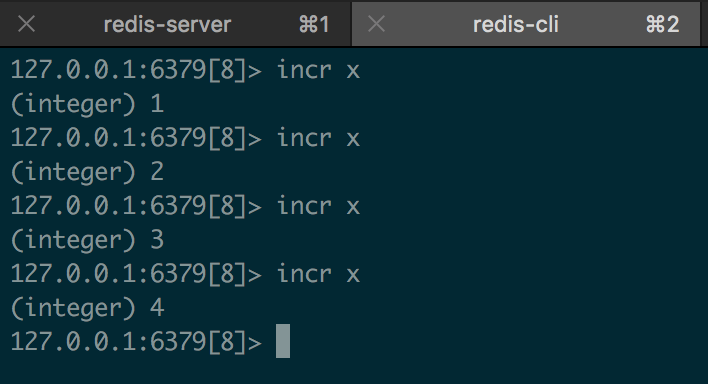
\includegraphics[scale=0.5]{img/pipe-incr}
\end{frame}

\begin{frame}[fragile]{Round Trip Time(RTT)}
  The round-trip delay time (RTD) or round-trip time (RTT) is the length of
  time it takes for a signal to be sent plus the length of time it takes for an
  acknowledgment of that signal to be received
  \footnote{\href{https://en.0wikipedia.org/index.php?q=aHR0cHM6Ly9lbi53aWtpcGVkaWEub3JnL3dpa2kvUm91bmQtdHJpcF9kZWxheV90aW1l}{Round Trip Time - Wikipedia}}.
\end{frame}

\begin{frame}[fragile]{Round Trip Time(RTT)}
  For instance if the RTT time is 250 milliseconds (in the case of a very slow
  link over the Internet), even if the server is able to process 100k requests
  per second, we'll be able to process at max four requests per second.

  If the interface used is a loopback interface\footnote{Loopback, or loop-back,
  refers to the routing of electronic signals, digital data streams, or flows of
  items back to their source without intentional processing or modification.
  \href{https://en.0wikipedia.org/index.php?q=aHR0cHM6Ly9lbi53aWtpcGVkaWEub3JnL3dpa2kvTG9vcGJhY2s}{Loopback - Wikipedia}},
  the RTT is much shorter (for instance my host reports 0,044 milliseconds
  pinging 127.0.0.1), but it is still a lot if you need to perform many writes
  in a row.

  Fortunately there is a way to improve this use case.
\end{frame}

\begin{frame}[fragile]{Redis Pipelining}
  It is possible to send multiple commands to the server without waiting for the
  replies at all, and finally read the replies in a single step.
\end{frame}

\begin{frame}[fragile]{Redis Pipelining}
  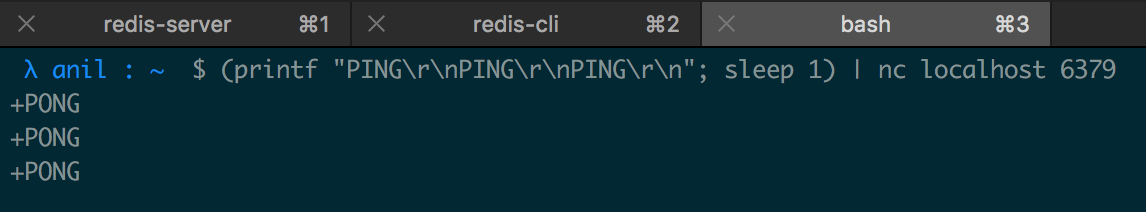
\includegraphics[scale=0.5]{img/pipelining}
\end{frame}

\begin{frame}[fragile]{Redis Pipelining}
  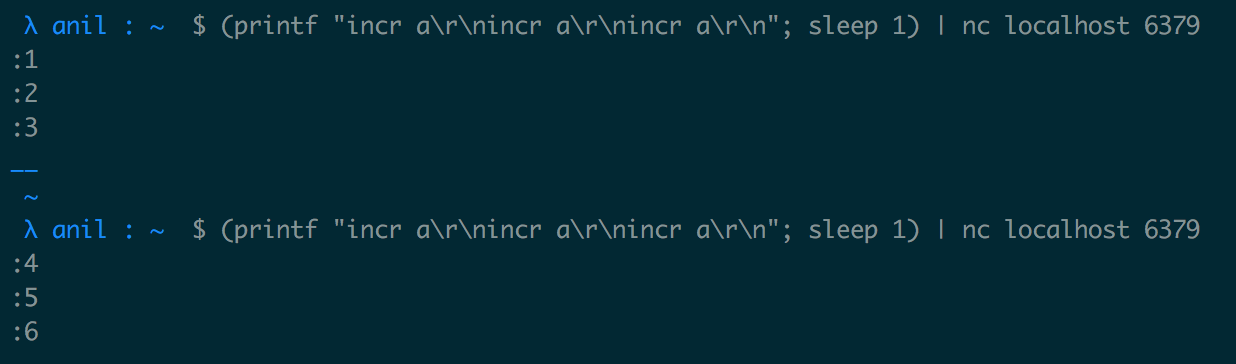
\includegraphics[scale=0.5]{img/pipelining-2}
\end{frame}

\begin{frame}[fragile]{Redis Pipelining in pyredis}
  \inputpython{redis.py}{1}{15}
\end{frame}

\begin{frame}[fragile]{Redis Pipelining}
  \begin{alertblock}{IMPORTANT NOTE:}
    \begin{itemize}
      \item While using pipelining, the server will be forced to queue the
      replies, using memory.
      \item So if you need to send a lot of commands with pipelining, it is
      better to send them as batches having a reasonable number, for instance
      10k commands, read the replies, and then send another 10k commands again,
      and so forth.
      \item The speed will be nearly the same, but the additional memory used
      will be at max the amount needed to queue the replies for this 10k commands.
    \end{itemize}
	\end{alertblock}
\end{frame}

\begin{frame}[fragile]{It's not just a matter of RTT}
  \begin{itemize}
    \item Without using pipelining, serving each command is very \textbf{cheap}
    from the point of view of accessing the data structures and producing the
    reply, but it is very \textbf{costly} from the point of view of
    \textbf{doing the socket I/O}.
    \item This involves calling the read() and write() syscall, that means going
    from user land to kernel land. The context switch
    \footnote{\href{https://en.0wikipedia.org/index.php?q=aHR0cHM6Ly9lbi53aWtpcGVkaWEub3JnL3dpa2kvQ29udGV4dF9zd2l0Y2g}{Context Switching - Wikipedia}}
    is a huge speed penalty.
    \item When pipelining is used, many commands are usually read with a
    \textbf{single} read() system call, and multiple replies are delivered with
    a \textbf{single} write() system call.
  \end{itemize}

\end{frame}

\begin{frame}[fragile]{It's not just a matter of RTT}
  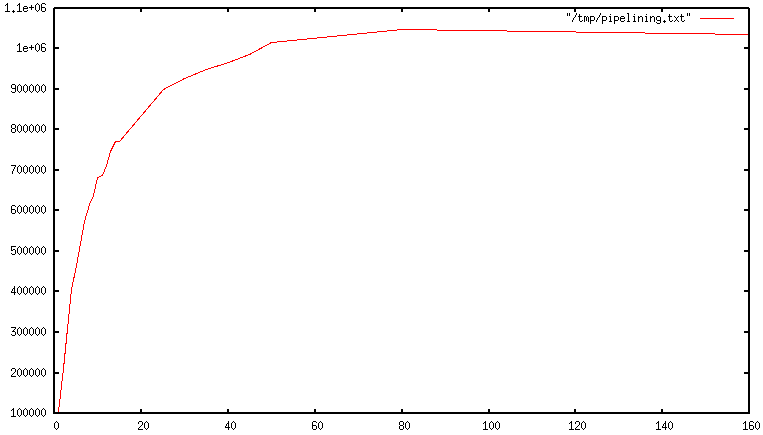
\includegraphics[scale=0.4]{img/pipeline_iops}
\end{frame}

\section{Redis Pub/Sub}

\begin{frame}[fragile]{Pub/Sub}
  Senders (publishers) are not programmed to send their messages to specific
  receivers (subscribers). Rather, published messages are characterized into
  \textbf{channels}, without knowledge of what (if any) subscribers there may
  be.
\end{frame}

\begin{frame}[fragile]{SUBSCRIBE}
  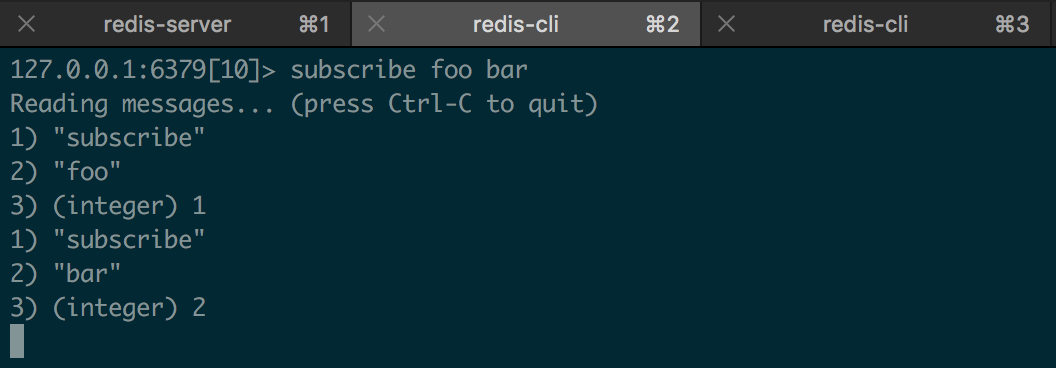
\includegraphics[scale=0.5]{img/subscribe}
\end{frame}

\begin{frame}[fragile]{SUBSCRIBE Cont...}
  \begin{itemize}
      \item A client subscribed to one or more channels should not issue
      commands, although it can subscribe and unsubscribe to and from other
      channels.
      \item The commands that are allowed in the context of a subscribed client
      are SUBSCRIBE, PSUBSCRIBE, UNSUBSCRIBE, PUNSUBSCRIBE, PING and QUIT.
  \end{itemize}
\end{frame}

\begin{frame}[fragile]{SUBSCRIBE Cont...}
  \begin{itemize}
    \item It is issued a subscription event for channels foo and bar, and both
    succeed.
    \item So, client at tab 2 is listening channels foo and bar.
    \item Let's publish some messages and see what happens.
  \end{itemize}
\end{frame}

\begin{frame}[fragile]{PUBLISH}
  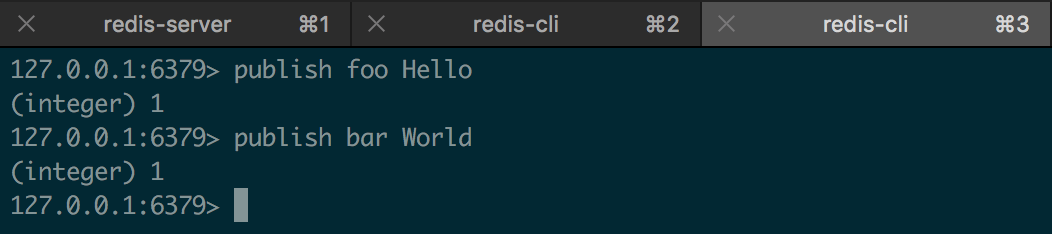
\includegraphics[scale=0.5]{img/publish}
\end{frame}

\begin{frame}[fragile]{Messages}
  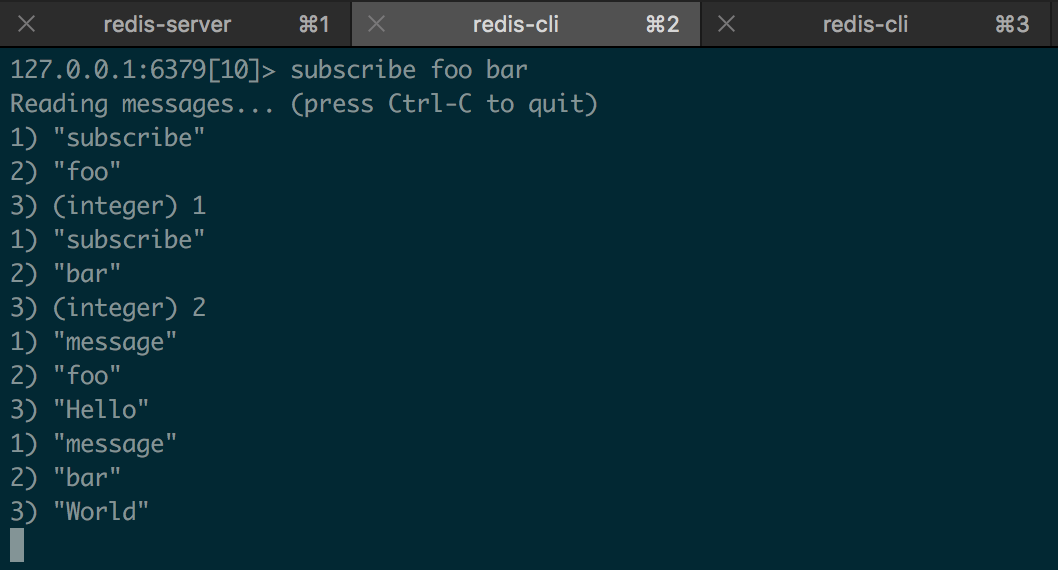
\includegraphics[scale=0.5]{img/subscriber-messages}
\end{frame}

\begin{frame}[fragile]{Messages Cont...}
  \begin{itemize}
    \item So, Hello is published to channel foo and World is published to
    channel bar.
    \item Subscriber client received the messages in a specific format.
  \end{itemize}
\end{frame}

\begin{frame}[fragile]{Messages Cont...}
  \begin{itemize}
    \item A message is an Array reply with three elements.
    \item The first element is the kind of message:
      \begin{itemize}
        \item \textbf{subscribe}: means that we successfully subscribed to the
        channel given as the second element in the reply. The third argument
        represents the number of channels we are currently subscribed to.
        \item \textbf{unsubscribe}: means that we successfully unsubscribed from
        the channel given as second element in the reply. The third argument
        represents the number of channels we are currently subscribed to. When
        the last argument is zero, we are no longer subscribed to any channel,
        and the client can issue any kind of Redis command as we are outside the
        Pub/Sub state.
        \item \textbf{message}: it is a message received as result of a PUBLISH
        command issued by another client. The second element is the name of the
        originating channel, and the third argument is the actual message
        payload.
      \end{itemize}
  \end{itemize}
\end{frame}

\begin{frame}[fragile]{Pattern-matching subscriptions}
  \begin{itemize}
    \item The Redis Pub/Sub implementation supports pattern matching.
    \item Clients may subscribe to glob-style patterns in order to receive all
    the messages sent to channel names matching a given pattern.
  \end{itemize}
\end{frame}

\begin{frame}[fragile]{PSUBSCRIBE}
  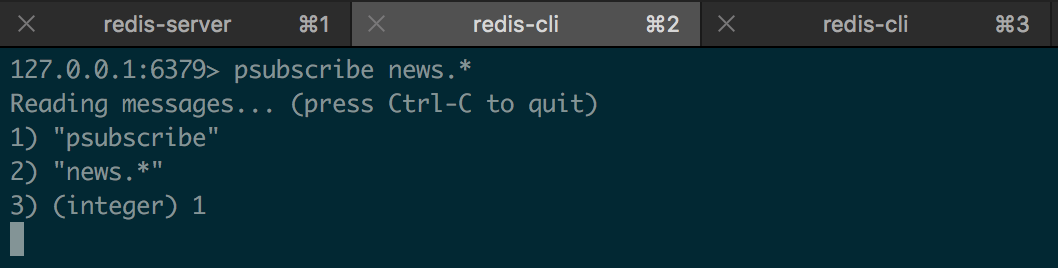
\includegraphics[scale=0.5]{img/psubscribe}
\end{frame}

\begin{frame}[fragile]{PSUBSCRIBE Cont...}
  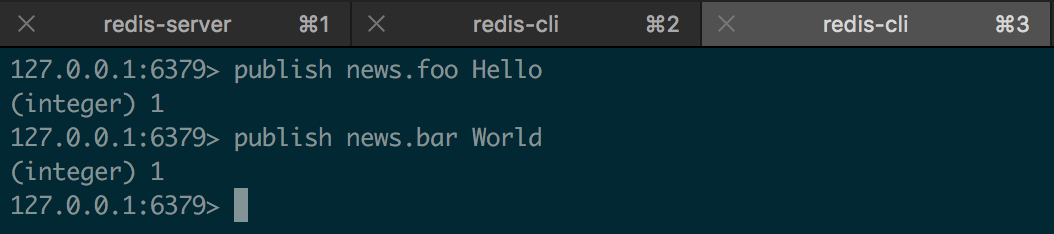
\includegraphics[scale=0.5]{img/publish-psubscribe}
\end{frame}

\begin{frame}[fragile]{PSUBSCRIBE Cont...}
  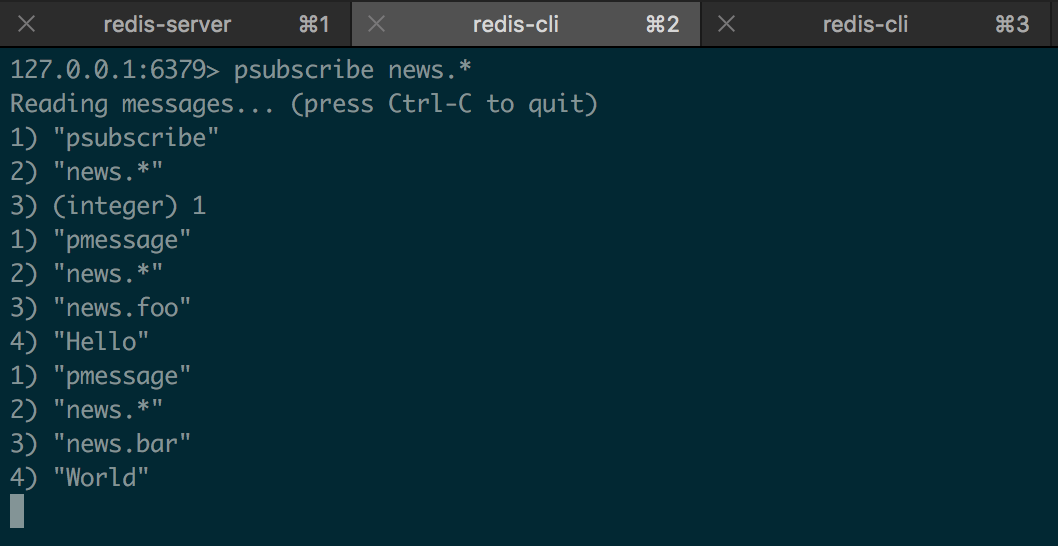
\includegraphics[scale=0.5]{img/psubscribe-message}
\end{frame}

\begin{frame}[fragile]{PMessage}
  Messages received as a result of pattern matching are sent in a different format:
  \begin{itemize}
    \item \textbf{pmessage}: it is a message received as result of a PUBLISH
    command issued by another client, matching a pattern-matching subscription.
    The second element is the original pattern matched, the third element is the
    name of the originating channel, and the last element the actual message
    payload.
  \end{itemize}
\end{frame}

\begin{frame}[fragile]{Redis Pub/Sub Conclusion}
  Redis gives a simple and handy usage of pub/sub pattern. Only thing to do is
  sending commands to it.
\end{frame}

\begin{frame}[fragile]{Questions}
  \inputpython{redis.py}{58}{65}
\end{frame}

\section{Demo}
\begin{frame}[fragile]{Demo - Vocabulary Application}
  Simple command line application that stores the words with their translations
  and give a chance to test user itself with pop-quiz option.
  \begin{itemize}
    \item add
    \item update
    \item read
    \item delete
    \item list
    \item quiz
  \end{itemize}

  Data-structures, pipelining and pub/sub mechanism are used.
\end{frame}

\section{Conclusion}
\begin{frame}[fragile]{Conclusion}
  Done.
  \begin{itemize}
    \item Data types
    \item Pipelining
    \item Pub/sub
  \end{itemize}
  Further.
  \begin{itemize}
    \item Keyspace Notifications
    \item Memory Optimization
  \end{itemize}
\end{frame}

\begin{frame}{Suggested Reading and Media}
  \begin{itemize}
    \item \href{https://www.infoq.com/presentations/Real-Time-Delivery-Twitter}{Real Time Delivery Twitter}
    \item \href{https://redis.io/commands/rpoplpush}{RPOPLPUSH}
    \item \href{https://redis.io/https://redis.io/commands/brpoplpush}{BRPOPLPUSH}
    \item \href{https://redis.io/topics/clients}{Redis Clients Handling}
    \item \href{https://redis.io/topics/notifications}{Keyspace Notifications}
    \item \href{https://redis.io/topics/memory-optimization}{Memory Optimization}
    \item \href{https://davidcel.is/posts/the-story-of-my-redis-database/}{Memory Optimization Case Story}
    \item \href{https://youtu.be/E708csv4XgY}{Messaging at Scale at Instagram}
  \end{itemize}
\end{frame}

\begin{frame}[fragile]{Contact}
  Find me on
  \begin{itemize}
    \item \href{https://github.com/anlcnydn}{github/anlcnydn}
    \item \href{https://twitter.com/anlcnydn}{twitter/anlcnydn}
  \end{itemize}
  or mail me at \href{mailto:anil@zetaops.io}{anil@zetaops.io}
\end{frame}

\begin{frame}{References}
  \begin{itemize}
    \item \href{https://redis.io/topics/data-types-intro}{Data Types}
    \item \href{https://redis.io/topics/pipelining}{Pipelining}
    \item \href{https://redis.io/topics/pubsub}{Pub/Sub}
    \item \href{https://redis.io/commands}{Commands}
  \end{itemize}
\end{frame}

\end{document}
